%------------------------------------------------------------------------------%

\usepackage{calculo_varias_variaveis-1}

\title {Gráficos e Curvas de Nível}

%------------------------------------------------------------------------------%
\begin{document}

\addtitle

%------------------------------------------------------------------------------%
\section{Gráfico de Uma Função Real}

%------------------------------------------------------------------------------%
\begin{frame}{Gráfico de uma Função Real}
  Conjunto de pontos $(x, y) \in \R^2$ tais que \(y = f(x)\)

  \pause
  \vspace{\baselineskip}
  Todos os pontos da forma
  \[
    \big( \, x, \, f(x) \, \big)
  \]
\end{frame}

%------------------------------------------------------------------------------%
\begin{frame}{Gráfico de uma Função Real}
  \centering
  

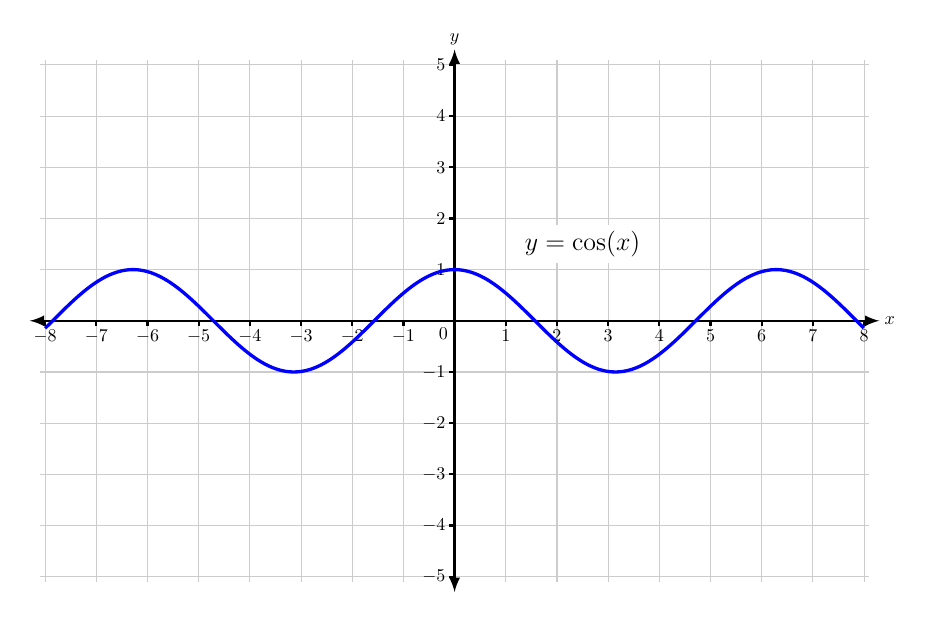
\begin{tikzpicture}[thick,scale=0.65, every node/.style={scale=0.65}]
  \def \minx {-8}
  \def \maxx {8}
  \def \miny {-5}
  \def \maxy {5}

  \draw[thin,black!20] (\minx-0.1,\miny-0.1) grid (\maxx+0.1,\maxy+0.1);

  \draw[thick, latex-latex] (\minx-0.3,0)--(\maxx+0.3,0);
  \draw[thick, latex-latex] (0,\miny-0.3)--(0,\maxy+0.3);
  \node at (\maxx+0.5,0) {$x$};
  \node at (0,\maxy+0.5) {$y$};

  \foreach \x in {\minx,...,-1}{
    \draw (\x,0)--(\x,-0.1);
    \node[below,black] at (\x,-0.05) {$\x$};
  }
  \foreach \x in {1,...,\maxx}{
    \draw (\x,0)--(\x,-0.1);
    \node[below,black] at (\x,-0.05) {$\x$};
  }
  \foreach \y in {\miny,...,-1}{
    \draw (0,\y)--(-0.1,\y);
    \node[left,black] at (-0.05,\y) {$\y$};
  }
  \foreach \y in {1,...,\maxy}{
    \draw (0,\y)--(-0.1,\y);
    \node[left,black] at (-0.05,\y) {$\y$};
  }
  \node[below left,black] at (0,0) {$0$};

  \draw[very thick, domain=\minx:\maxx, variable=\x, smooth, samples=300, blue]  plot ({\x},{cos(\x r)});

  \node at (2.5,1.5) [fill=white] {\Large $y=\cos(x)$};
\end{tikzpicture}

\end{frame}

%------------------------------------------------------------------------------%
\section{Gráfico de Uma Função de Duas Variáveis}

\begin{frame}{Gráfico de Uma Função de Duas Variáveis}
  Dada uma função \(f\colon\R^2\to\R\)
  \begin{itemize}[<+->]
    \item Gráfico de $f$, ou superfície \(z=f(x, y)\) \\
    é o conjunto de pontos
    \[
      \big( \, x, \, y, \, f(x, y) \, \big)
    \]
  \end{itemize}
\end{frame}

%------------------------------------------------------------------------------%
\section{Gráfico de Uma Função de Várias Variáveis}

\begin{frame}{Gráfico de Uma Função de Duas Variáveis}
\end{frame}

%------------------------------------------------------------------------------%
\section{Lista Mínima}

%------------------------------------------------------------------------------%
\begin{frame}{Lista Mínima}
  Cálculo Vol. 2 do Thomas 12\textsuperscript{a} ed. -- Seção 14.1
  \begin{enumerate}
    \item Estudar o texto da seção
    \item Resolver os exercícios:
  \end{enumerate}

  \vfill
  Atenção: A prova é baseada no livro, não nas apresentações
\end{frame}

%------------------------------------------------------------------------------%
\end{document}
%------------------------------------------------------------------------------%
